%% LyX 2.2.2 created this file.  For more info, see http://www.lyx.org/.
%% Do not edit unless you really know what you are doing.
\documentclass[british,english]{article}
\usepackage[T1]{fontenc}
\usepackage[latin9]{luainputenc}
\usepackage[a4paper]{geometry}
\geometry{verbose,tmargin=2cm,bmargin=2cm,lmargin=2cm,rmargin=2cm}
\setlength{\parindent}{0bp}
\usepackage{array}
\usepackage{float}
\usepackage{multirow}
\usepackage{algorithm2e}
\usepackage{graphicx}

\makeatletter

%%%%%%%%%%%%%%%%%%%%%%%%%%%%%% LyX specific LaTeX commands.
%% Because html converters don't know tabularnewline
\providecommand{\tabularnewline}{\\}

\@ifundefined{showcaptionsetup}{}{%
 \PassOptionsToPackage{caption=false}{subfig}}
\usepackage{subfig}
\makeatother

\usepackage{babel}
\begin{document}

\title{\hrulefill \\ 
\textbf{Technical Progress Report} \\ 
F-CER54-3: Using machine learning to control an inverted double pendulum using camera feedback\\ 
\vspace{0.2cm} 
\normalsize  Nicholas Capel (nrjc2) \\ 
\normalsize Supervisor: Prof. Carl Edward Rasmussen \\
\hrulefill \\}
\maketitle
\begin{abstract}
The aim of this project is to implement the control of an inverted
double pendulum in the PILCO framework using camera feedback. Work
to date has involved MATLAB computer simulation experiments to understand
how added delay and uncertainty about states can adversely affect
training of the model and controller parameters in the PILCO framework.
Additional work was done to determine an upper bound on the system
delay introduced by processing times and video lag. Going forward,
a physical system of the double pendulum will be implemented. Furthermore,
experiments will be conducted on a SIMULINK model to better understand
the problem from a control perspective, and the camera experiments
will be refined.
\end{abstract}

\section{Introduction}

The inverted double pendulum problem is a control problem.

\begin{figure}[H]
\caption{Diagram of setups}

\subfloat[Problem setup]{
\centering{}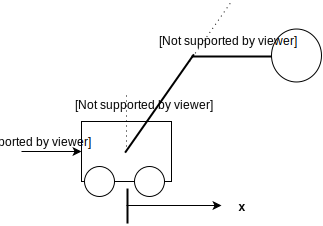
\includegraphics[width=0.5\textwidth]{diag/pendulum}}\subfloat[System setup]{
\centering{}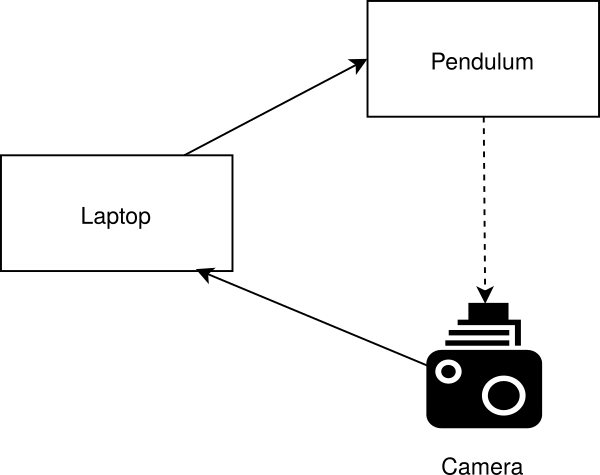
\includegraphics[width=0.5\textwidth]{diag/experimentalsetup}\label{systemsetup}}
\end{figure}

The state of the system is described by $x$. 

\[
x=[\dot{x_{t}},x_{t},\dot{\theta_{1(t)}},\theta_{1(t)},\dot{\theta_{2(t)}},\theta_{2(t)}]^{T}
\]

The objective of the control problem is to discover a controller to
minimize the expected cost function over an infinite time horizon.
In this project, the PILCO framework is used to both discover a model
of the system, and to design a controller to stabilize the system
\cite{Rasmussen}. 

In reality, this corresponds to the pendulum performing two tasks:
\begin{enumerate}
\item Swing up: The pendulum is initialised at the position $\theta_{1}=\pi,\,\theta_{2}=0$
. The control system has to swing the pendulum up such that $\theta_{1}=0$
\item Stabilize: The controller has to control the system state such that
$\theta_{1}=0,\,\theta_{2}=0$
\end{enumerate}
In this project, another layer of difficulty is added. The current
state vector of the system, $x$, cannot be directly read from sensors,
but must be inferred from a video feed. Thus, the apparatus is set
up as shown in Figure \ref{systemsetup}.

\section{Motivation and Theory}

The classical approach to the Inverted Double Pendulum problem involves
writing down the Newtonian equations and making a first order approximation
about the equilibrium point. However, this model-based approach fails
when the linear approximation breaks down, and it is difficult to
exactly characterise this point of failure. Thus, successful approaches
to the problem of both swing up and stabilization involve defining
multiple equilibrium states that can be linearized, and designing
a controller to successfully transition between these states\cite{pendulum}.

\begin{figure}[H]
\caption{PILCO algorithm}

\subfloat[overview]{
\centering{}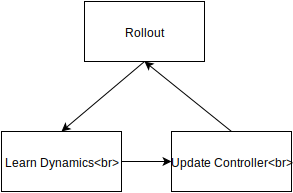
\includegraphics[width=0.5\textwidth]{diag/pilcooverview}\label{pilcooverview}}\subfloat[rollout]{
\centering{}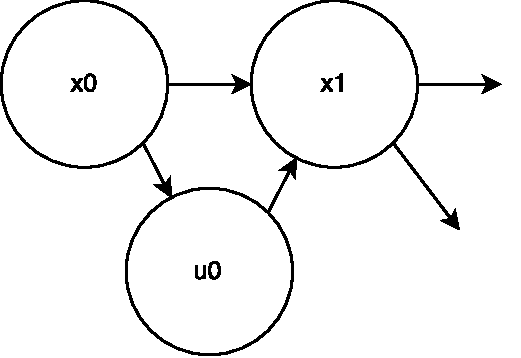
\includegraphics[width=0.5\textwidth]{diag/rollout}\label{pilcorollout}}
\end{figure}

The PILCO approach is to use a data-based approach to learn a Gaussian
Process model that describes the transition from $x_{t}\rightarrow x_{t+1}$.
The Gaussian Process can model both the transition between the two
states, as well as give an uncertainty estimate about the transition.
By propagating the state forward in time, as in Figure \ref{pilcorollout},
a cost function can be made: 
\[
c=\sum_{t=0}^{T}E[f(x_{t})]
\]

We can thus perform gradient descent over the cost function, which
is parameterized by the controller parameters, to obtain an optimal
controller to perform the stabilization task. 

In each iteration of the PILCO algorithm (Figure \ref{pilcooverview}),
a GP dynamics model is learned using all previous data, and a cost
function is minimized to discover the optimal controller policy. After
which, the controller policy is applied to a real system (a rollout),
and the algorithm repeats. 

Stabilization of the inverted double pendulum has been attempted before,
without success\cite{Kukla}. This is becasue noise and uncertainty
about the pendulum state has significantly affected the ability of
the PILCO algorithm to learn both the controller and system dynamics. 

\section{Progress and Results}

\subsection{Computer Simulations: Stabilization About Equilibrium Point}

The first objective is to discover if the problem is tractable. How
much delay and noise can be added to the system before the PILCO algorithm
fails?

A computer model of the double pendulum was built by simulating Newton's
equations in MATLAB. PILCO is then used on the simulated double pendulum,
initialized with varying levels of noise and delay, and the results
are \foreignlanguage{british}{analysed} to understand if the PILCO
control problem is tractable. 

In this series of experiments, a linear policy model was chosen for
the control, and the initial state of the system is set such that
$\theta_{1}\approx0,\,\theta_{2}\approx0$. In previous experiments\cite{Kukla}
with the PILCO algorithm, the controller was able to perform swingup,
but was unable to stabilize the penduli about the equilibria. Hence,
it is appropriate to investigate the failure of the PILCO algorithm
about the $\theta_{1}\approx0,\,\theta_{2}\approx0$ point. 

A linear policy model was selected because it is the simplest controller
that can achieve the task, and is used in traditional control theory
approaches \cite{pendulum}. 

The Figure below represents a typical result of the attempted PILCO
stabilization

\begin{figure}[H]
\caption{GP predictions}

\subfloat[Base]{
\centering{}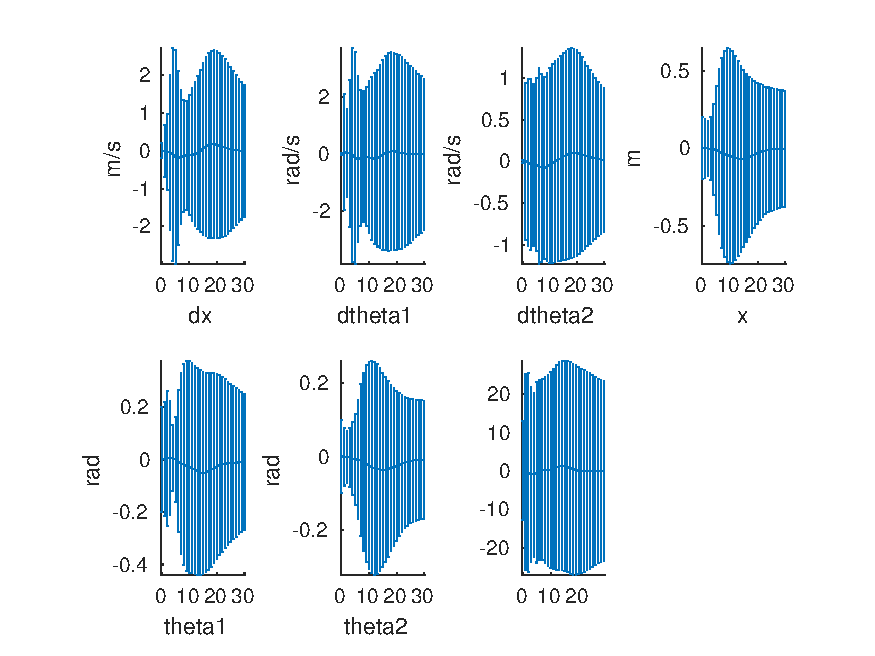
\includegraphics[width=0.5\textwidth]{diag/sampleRun2}\label{gpbase}}\subfloat[With rollouts]{
\centering{}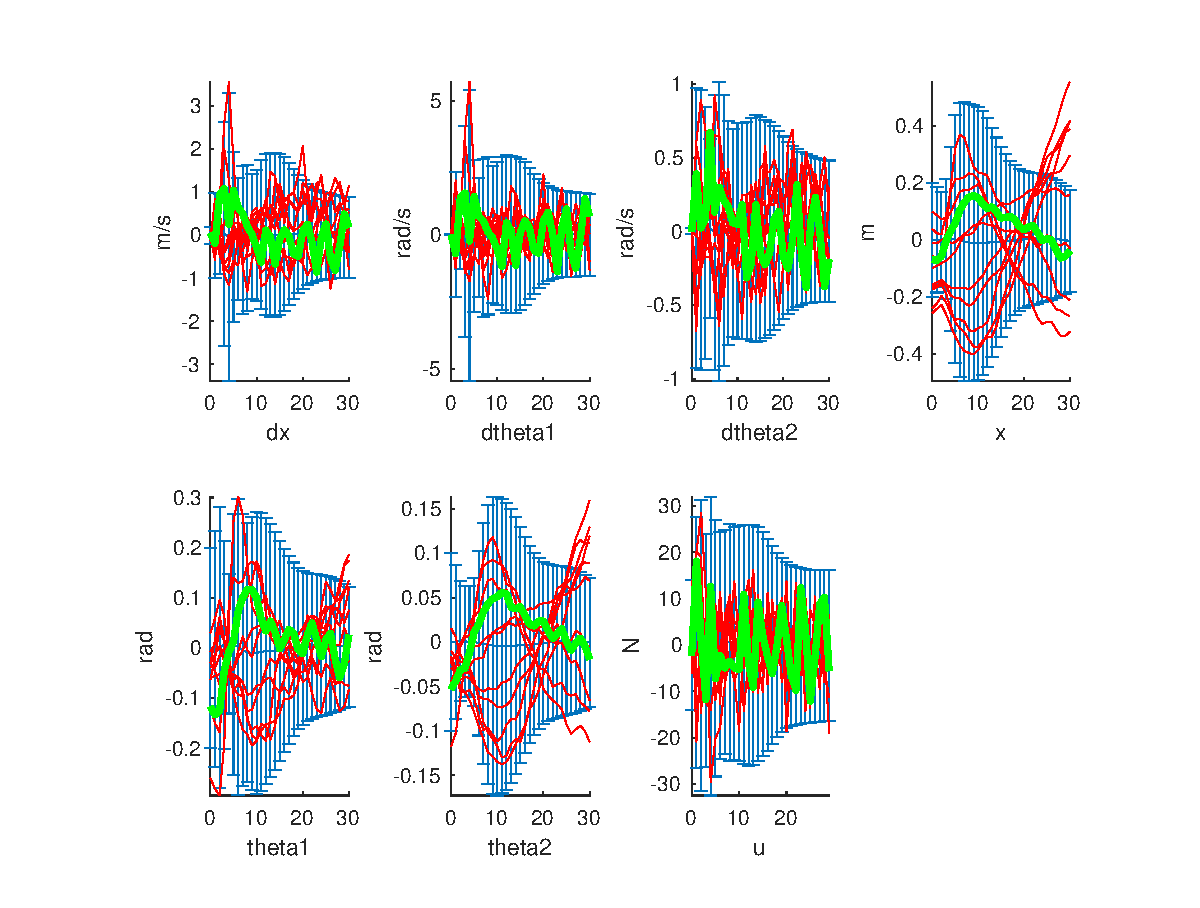
\includegraphics[width=0.5\textwidth]{diag/sampleRun}\label{gprollout}}
\end{figure}

The blue mean line (Figure \ref{gpbase}) represents the predicted
trajectory of the inverted double pendulum given the controller. The
blue bars represent the uncertainty or variance about this trajectory. 

The green line (Figure \ref{gprollout}) represents a rollout that
is observed by the PILCO framework. 

The red lines (Figure \ref{gprollout}) represent simulated rollouts.
These rollouts are drawn for display purposes, to evaluate the performance
of the PILCO framework, but the results obtained are not fed in to
the training of the GP. 

After plotting the results of the PILCO experiments, the next step
is to find a method to evaluate the performance of the PILCO framework.
The PILCO framework can fail in two ways:
\begin{enumerate}
\item Model error: The framework learns an incorrect dynamics model.
\item Control error: The framework learns the correct dynamics model, but
cannot discover a controller to control the unstable system. 
\end{enumerate}
If the control problem is tractable, two things should be observed.
First, as the number of steps increases, the predicted trajectory
should be centered on the targeted state, and the variance of the
trajectory should be tightly bound. This demonstrates that there is
no control error. 

Secondly, the trajectories of the simulated and actual rollouts should
be well described by the PILCO framework. 

In an initial series of experiments, single trials were conducted
for various delays and noise scaling factors. To model random noise,
the computer setup corrupts the observation of each state by sampling
from a Gaussian centered about the true value with a variance. The
noise scaling factor scales this variance to model different magnitudes
of noise. 

\begin{figure}[H]
\caption{Stability}

\centering{}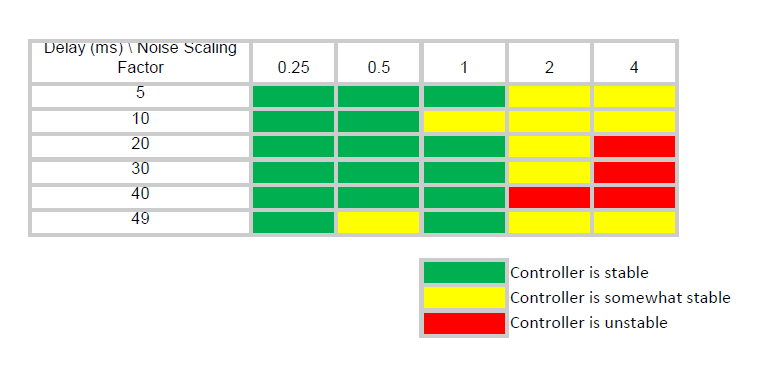
\includegraphics[width=0.7\textwidth]{diag/stability}
\end{figure}

The results are promising, suggesting that the PILCO algorithm is
more strongly affected by noise than by delays. However, the analysis
of the stability is crude: manual observation and classification of
the trajectories is used to determine whether a controller is stable,
somewhat stable, or unstable.

The experiment was then repeated 4 times, and a simple algorithm was
used to quantify the stability of a single PILCO trial. A trial is
initially assigned a stability rating of 0 (the most stable). When
certain conditions are fulfilled, penalty points are added to the
stability rating.

\begin{table}[H]
\caption{Stability Rating}

\centering{}%
\begin{tabular}{|>{\centering}p{0.4\textwidth}|c|>{\raggedright}p{0.4\textwidth}|}
\hline 
Condition (evaluated for state variable $\theta_{2}$) & Penalty & Reasoning\tabularnewline
\hline 
\hline 
$\sigma(T_{max})>\sigma(T_{max-1})>\sigma(T_{max-2})$  & 1 & System state unbound $\longrightarrow$control error\tabularnewline
\hline 
$\theta_{2}(actual)>\theta_{2}(pred)+2\sigma$ or\linebreak{}
$\theta_{2}(actual)<\theta_{2}(pred)-2\sigma$ \linebreak{}
for $>3/10,\,<7/10$runs & 1 & \multirow{2}{0.4\textwidth}{Rollouts not well described by model $\longrightarrow$model error}\tabularnewline
\cline{1-2} 
$\theta_{2}(actual)>\theta_{2}(pred)+2\sigma$ or\linebreak{}
$\theta_{2}(actual)<\theta_{2}(pred)-2\sigma$ \linebreak{}
for $>7/10$runs & 2 & \tabularnewline
\hline 
\end{tabular}
\end{table}

Thus, an average stability rating can be computed for all 5 runs. 

\begin{figure}[H]
\caption{Average stability rating over 5 runs}

\centering{}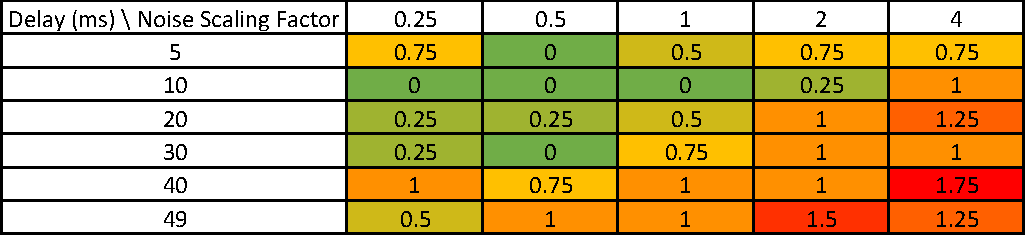
\includegraphics[width=0.7\textwidth]{diag/stabilityFull}
\end{figure}

Once again, the trend identified in the original experiment does not
disappear: the PILCO algorithm seems to be more strongly affected
by noise than by delays. 

\subsection{Camera Experiment}

An experiment was conducted using a program written in Java to estimate
the magnitude of the camera delay. 
\begin{enumerate}
\item Camera and LED are placed in dark room.
\item LED is turned on, timing begins. 
\item When camera observes an increase in brightness, stop timing. 
\end{enumerate}
This experiment aims to discover the minimum time taken for an output
of the system to propagate to the input. Hence, the time recorded
in this experiment should serve as an upper bound on the size of the
delay. Repeating the experiment, it appears that:

\[
t_{delay}(max)=(307\pm60)ms
\]

Originally, it was hypothesized that the delay is on the order of
30ms. However, the delays obtained in this experiment were a full
order of magnitude higher. However, the delay found in this experiment
is an upper bound on the delay and not the actual delay. Hence, the
actual delay will probably be far lower.

\section{Future Plans}

\subsection{Control Theory Perspective}

A model will be created in SIMULINK to model an optimal linear controller
for the inverted double pendulum as well as the system itself. Experiments
will be conducted with varying time delays and noise levels in this
system to understand if the control problem is tractable using the
best methods under noisy conditions with delay. 

\subsection{Further Camera Experiments}

More experiments will be conducted with the camera system to obtain
both a lower bound as well as upper bound of the delay. Additionally,
the experiment will be redone in C++ / C (which the actual system
will be written in), to increase the speed of processing and to reduce
the size of the delay. 

\subsection{Variance Experiments}

Initial experiments suggest that the PILCO algorithm is more strongly
affected by noise than by delays. Given that, further experiments
will be conducted to discover which of the 7 state variables $x$
will most severely affect the stability of the PILCO algorithm. To
this end, the simulation experiment will be conducted. However, unlike
the original, instead of introducing a noise scaling term to scale
the noise corrupting all 6 state variables simultaneously, the total
variance will instead be kept constant and only the distribution amongst
the 6 state variables will vary. 

\subsection{Physical Implementation}

After this is done, the C++ code will be written, calling on OpenCV
libraries in order to implement the PILCO algorithm for a physical
system. If it is discovered that delays or noise levels are too high
to implement a system controlled using visual feedback, the camera
will be replaced in \foreignlanguage{british}{favour} of either a
faster camera, or for actual sensors on the joints of the physical
system. 
\begin{thebibliography}{1}
\bibitem{Rasmussen}Deisenroth, Marc, and Carl E. Rasmussen. \textquotedbl{}PILCO:
A model-based and data-efficient approach to policy search.\textquotedbl{}
Proceedings of the 28th International Conference on machine learning
(ICML-11). 2011.

\bibitem{pendulum}Yamakita, M. A. S. A. K. I., et al. \textquotedbl{}Robust
swing up control of double pendulum.\textquotedbl{} American Control
Conference, Proceedings of the 1995. Vol. 1. IEEE, 1995.

\bibitem{Kukla}Kukla, M. M. (n.d.). Learning to control double inverted
pendulum with vision feedback. 
\end{thebibliography}

\end{document}
